\documentclass[a4paper, twocolumn]{article}
\usepackage[paper=a4paper, centering, margin=2cm]{geometry}
\usepackage{pgfornament}
\usepackage{everypage}
\usepackage{graphicx}
\usepackage{lipsum}
\usepackage{linguex}
\usepackage{glossaries}
\usepackage{array}
%\usepackage{supertabular}
\usepackage{nopageno}
\usepackage{hyperref}
\usepackage{fouriernc} % Use the New Century Schoolbook font


\def\PageTopMargin{2cm}
\def\PageLeftMargin{2cm}
\newcommand\atxy[3]{%
 \AddThispageHook{\smash{\hspace*{\dimexpr-\PageLeftMargin-\hoffset+#1\relax}%
  \raisebox{\dimexpr\PageTopMargin+\voffset-#2\relax}{#3}}}}

\usepackage{chngcntr}
\counterwithin{ExNo}{section}
\renewcommand{\ExLBr}{\bfseries}
\renewcommand{\ExRBr}{}
\renewcommand{\Exarabic}{\thesection.\arabic} 

\newcommand{\fixedlabel}[1]{\textbf{\makebox[3.5em][l]{#1}}}

% \setlength{\Extopsep}{.66\baselineskip}
% \newlength{\testspace}
% \setlength{\itemspace}{.66\baselineskip}

\newcommand{\itemspace}{\vspace{1.2mm}\\}
\newcommand{\placeframe}[1]{\atxy{-0.5cm}{29.1cm}{\includegraphics[scale=0.3353]{images/frame#1}}}



\definecolor{titlegreen}{RGB}{12, 86, 65}
\definecolor{pooltablegreen}{RGB}{98, 166, 111}  % same colour as the pool table diagram

\title{Pilaar Duncan Pool House Rules}
\author{Leo Duncan}

\hypersetup{
    pdftitle={Pool Rulebook},
    pdfsubject={The Pilaar Duncan Family Pool Rules are the house rules for pool developed by and for the Pilaar Duncan family.},
    pdfauthor={Leo Duncan},
    allbordercolors={pooltablegreen}
}

\newcommand{\currentversion}{3.0}
\newcommand{\currentversiondate}{13 July 2025}



\begin{document}

\begin{titlepage}
	
    \placeframe{0}

	\centering % Centre everything on the title page
	
    % idk copied this from a titlepage template and this gives good spacing so not messing with it.
	\textcolor{white}{\rule{\textwidth}{1pt}} % Thick horizontal rule
	\vspace{2pt}\vspace{-\baselineskip} % Whitespace between rules
	\textcolor{white}{\rule{\textwidth}{0.4pt}} % Thin horizontal rule
	\vspace{0.1\textheight} % Whitespace between the top rules and title
	
	%------------------------------------------------
	%	Actual text below here
	%------------------------------------------------
	
	\textcolor{titlegreen}{\LARGE Pilaar Duncan Family}\\[0.5\baselineskip] % Title line 1
	\textcolor{titlegreen}{\Huge Pool Rules}\\[0.5\baselineskip] % Title line 2
    %\textcolor{titlegreen}{\Large \& Variations}\\[0.5\baselineskip] % Title line 3
	
	\vspace{0.025\textheight} % Whitespace between the title and short horizontal rule
	\rule{0.3\textwidth}{0.4pt} % Short horizontal rule under the title
	\vspace{0.1\textheight} % Whitespace between the thin horizontal rule and the author name
	
	{\large \textit{Developed By}}\\[0.75\baselineskip] % Author name
    {\Large \textsc{Chris Duncan, Leo Duncan, Lily Duncan,}}\\[0.5\baselineskip]
    {\Large \textsc{Tom Duncan, Carla Pilaar, \& Mark Pilaar}}\\[0.5\baselineskip]

    \vspace{3\baselineskip}

    {\large \textit{Compiled By}}\\[0.75\baselineskip] % Author name
    {\Large \textsc{Leo Duncan}}\\[0.5\baselineskip]

    \vfill

    {\normalsize \textit{Version \currentversion}}
	
\end{titlepage}

\placeframe{1}

% maybe consider adding a Section 0: General Description as in https://poolplayers.com/8-9-ball-Rules.pdf

\section{Format of Games} \label{format}
\ex. Games are generally played in a best-of-one, best-of-three, or best-of-seven format.\itemspace
\fixedlabel{1.1.1}Best-of-one matches are common when the players feel like a game but not too much of a commitment. This format sees whoever wins the game win overall.\itemspace
\fixedlabel{1.1.2}Best-of-three matches are the most common. The first player to win two games wins overall.\itemspace
\fixedlabel{1.1.3}Best-of-seven matches are usually the format for multi-day or holiday-long tournament-style competitions. In this, the first player to win four games wins overall. This format is more common in the Doubles variation of play (see \hyperref[doubles]{Section \ref*{doubles}}).
\par

\section{Racking} \label{racking}
\ex. Racking up the balls involves setting all 15 balls up in the standard triangle formation for the opponent to break. The opponent is encouraged to make sure the rack is tight.\par
\ex. \label{challengerracks}Determining Who Racks: The general rule is “challenger racks,” i.e., the person who challenged their opponent racks the balls. For example, if a player says, “Do you want a game?” they are the challenger, and thus they rack the balls. This general rule also extends to after each match. If a rematch is desired, the loser of the previous game is the challenger, and thus, they rack the balls.\par
\ex. \label{rackpos}Formation and Position of Rack:
    \begin{figure}[!h]
        \raggedleft
        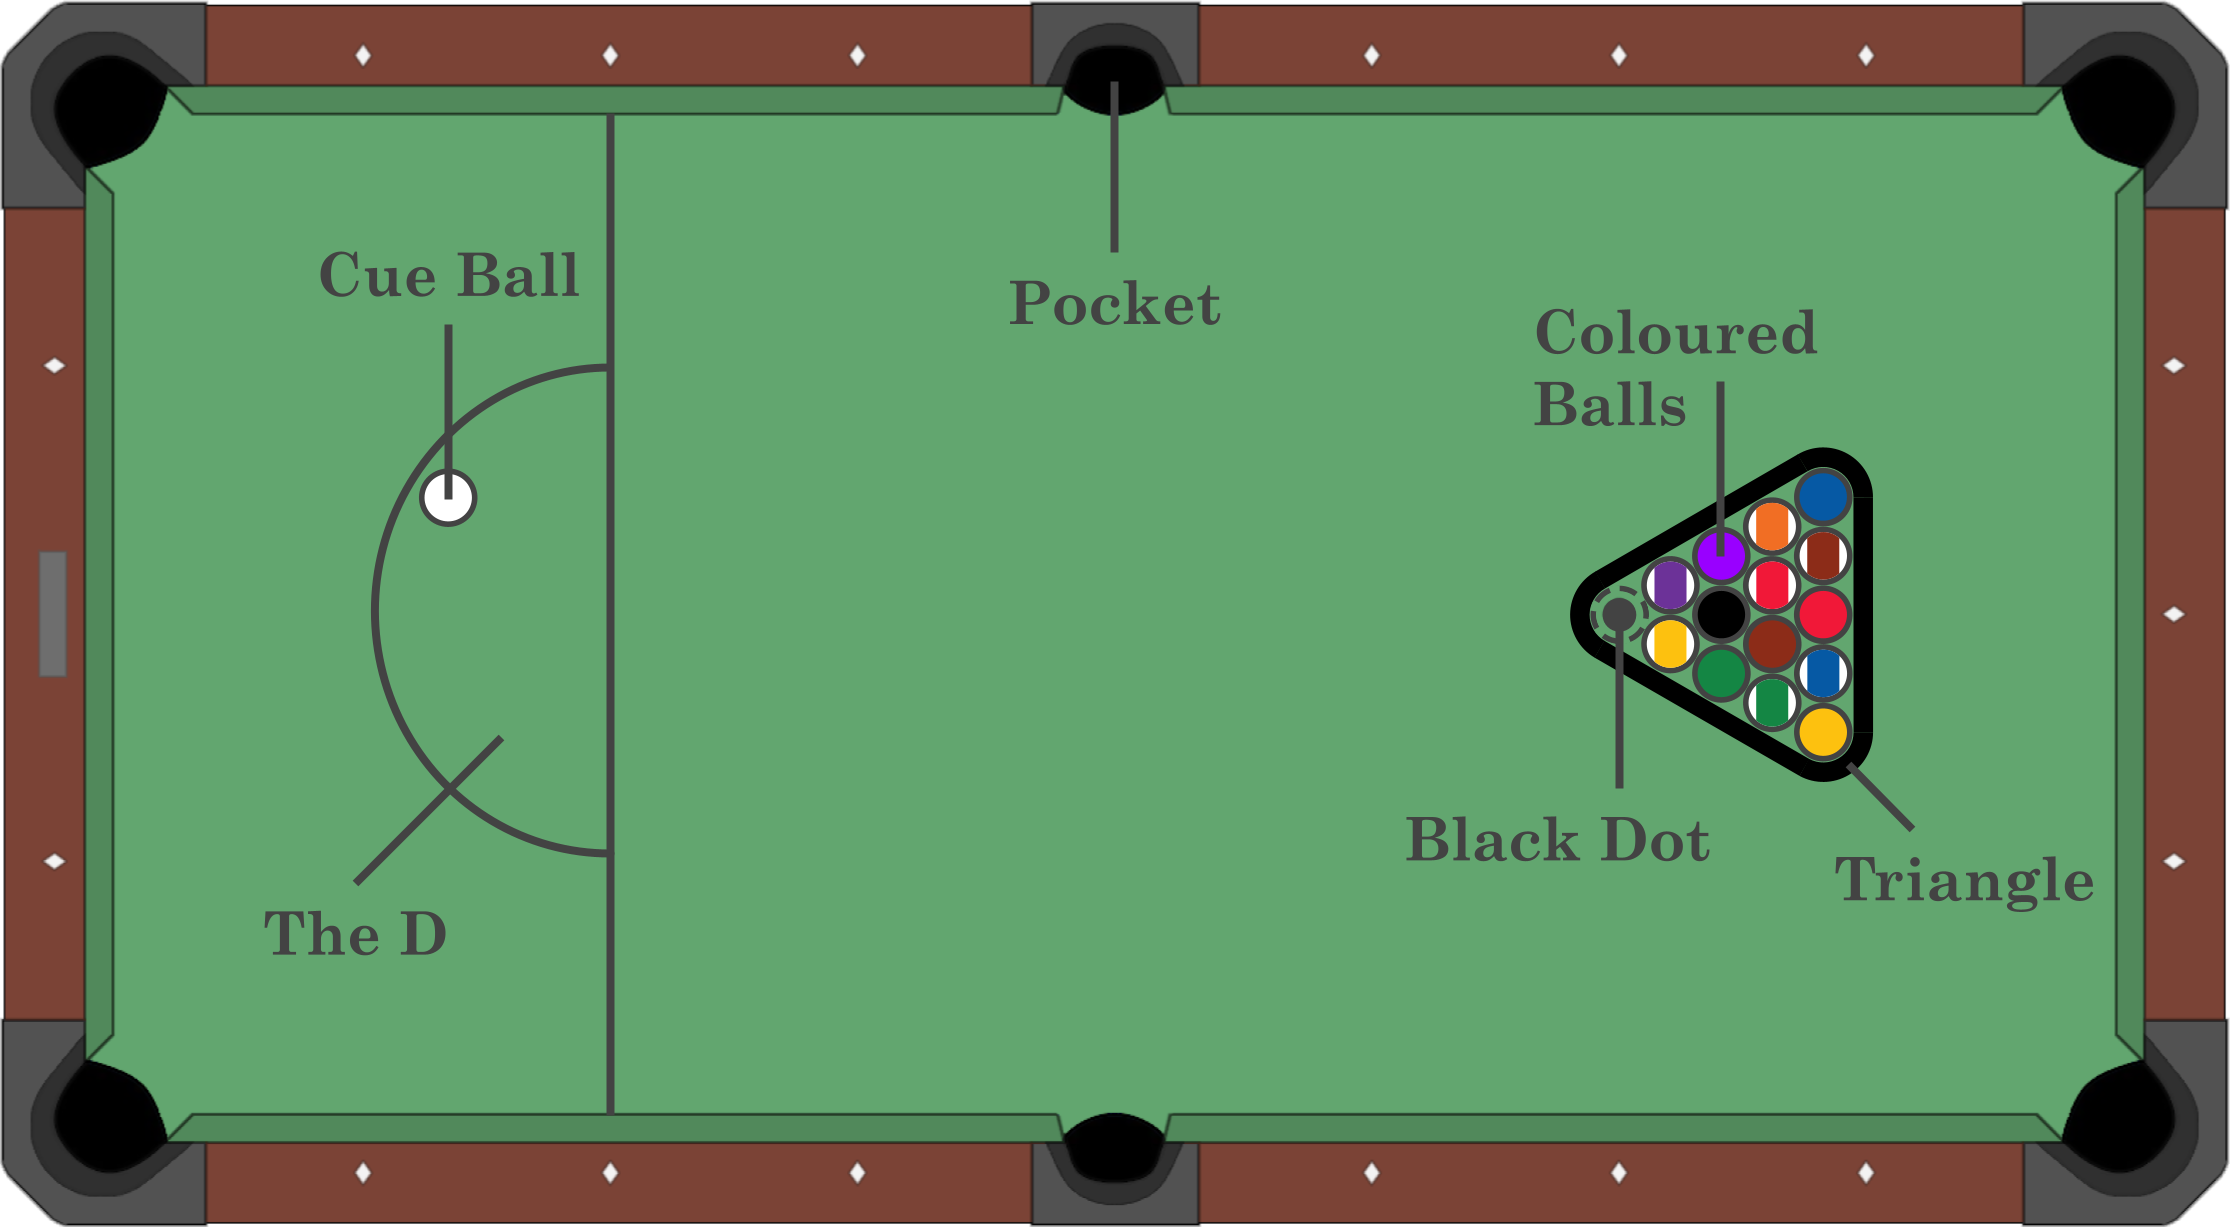
\includegraphics[width=0.4315\textwidth]{images/table_diagram.png}
        \hspace{-1.7mm}
        \label{fig:f1}
    \end{figure}\\
\fixedlabel{2.3.1}The 15 numbered balls are racked in a triangle with the black/8-ball in the centre (i.e., middle of the third row). Other than the black/8-ball, there is no required pattern for the order of the balls.\itemspace
\fixedlabel{2.3.2}The player racking needs to ensure that all the balls are tightly packed with no gaps.\itemspace
\fixedlabel{2.3.3}The triangle points towards the front of the table (where the opponent breaks from), with the front-most ball centred on top of the black dot.\itemspace
\fixedlabel{2.3.4}If a triangle racking tool is used, this is removed once the balls are in place. If the balls move when the triangle is removed, it should be placed back on, squishing the balls back together.\itemspace
\fixedlabel{2.3.5}The opponent breaking may inspect the rack for gaps and the position of the black/8-ball, but may not complain about the pattern of the coloured balls.
\par

\section{Breaking \& Establishment of Set} \label{breaking}
\ex. The player breaking places the cue ball in the D.\par
\ex. The player breaking has the right to “Call the Break” (see \hyperref[callingthebreak]{Section \ref*{callingthebreak}}). This is optional. Remembering to do this is the player's responsibility.\par
\ex. \label{breakingballs}The player breaking may hit the cue ball into any part of the rack, although hitting the front-most ball is typically recommended.\par
\ex. If the player breaking completely misses the rack but the cue ball remains on the table, they may pick up the cue ball and have one more attempt, provided no other ball has moved. If the cue ball sinks or bounces off the table, this is a foul and the break is handed to the opponent. A second failed attempt will also see the break handed to the opponent. In either instance, the opponent may not “Call the Break”.\par
\ex. If the cue ball hits a rail before hitting the rack, this is a foul.\par
\ex. If the cue ball hits the rack and ends up sinking, this is a foul.\par
\ex. If any balls get knocked off the table during the break, this is a foul. See \hyperref[ballofftable]{Section \ref*{ballofftable}.10} for returning the balls to the table.\par
\ex. If a coloured ball is sunk off the break, that set is the player's balls (i.e., overs or unders). The player can then take their next shot.\par
\ex. If multiple coloured balls from different sets are sunk off the break, the player chooses which set to play. The player can then take their next shot.\par
\ex. \label{breakingnoballs}If no balls are sunk off the break:\itemspace
\fixedlabel{3.10.1}At this stage, neither player has a set that belongs to them. The players will alternate turns to hit any coloured ball (not the black/8-ball) until a ball is sunk and sets are assigned.\itemspace
\fixedlabel{3.10.2}If the black/8-ball is hit first, this is a foul.\itemspace
\fixedlabel{3.10.3}If multiple balls from different sets are sunk off the same shot, whichever went in first is the set assigned to the player. If neither player saw which ball sunk first, the player chooses their set. No foul is awarded and the player can continue their turn.
\par
\ex. \hspace{-2.6mm} If the black/8-ball sinks off the break, this is an \\ \phantom{} \hspace{-2.5mm}instant loss.\par

\section{General Play} \label{general}

\ex. A player's turn consists of them striking the cue ball into their coloured balls, typically with the goal of sinking them.\par
\ex. The player must strike the cue ball with at least one foot on the floor. “Tippy toes” are permissible.\par
\ex. If the opponent fouled on their turn, then the player gets an additional shot (see \hyperref[fouling]{Section \ref*{fouling}} for more on fouls).\par
\ex. If a player sinks all of their coloured balls, they can now hit the black/8-ball with the cue ball directly.\par
\ex. The players alternate turns until the game is ended. See \hyperref[ending]{Section \ref*{ending}} for the ending of the game.

\placeframe{2}

\section{Fouling} \label{fouling}
\ex. If a foul occurs, then the player's turn ends, and the opponent is granted an extra shot in their turn.\par
\ex. Fouls do not stack. For example, if a player misses all balls and sinks the white, the opponent still only gets one extra shot.\par
\ex. Circumstances that give rise to fouls are as follows:\itemspace
\fixedlabel{5.3.1}The cue ball is hit into a ball that is not the player's own first. This does not include coloured balls being hit during the break (\hyperref[breakingballs]{Section \ref*{breakingballs}}) or during any subsequent shots until a ball sinks (\hyperref[breakingnoballs]{Section \ref*{breakingnoballs}}). Hitting the black/8-ball first remains a foul in these instances. This rule is excepted in some cases of a snooker (\hyperref[snooker]{Section \ref*{snooker}}).\itemspace
\fixedlabel{5.3.2}The cue ball does not hit any ball.\itemspace
\fixedlabel{5.3.3}The player sinks the cue ball.\itemspace
\fixedlabel{5.3.4}The player sinks an opponent's ball.\itemspace
\fixedlabel{5.3.5}During the break the cue ball hits a rail before hitting the rack.\itemspace
\fixedlabel{5.3.6}The player strikes the cue ball while any ball on the table is still moving.\itemspace
\fixedlabel{5.3.7}The player fails a nomination while attempting to escape some forms of a snooker (see \hyperref[snooker]{Section \ref*{snooker}}).\itemspace
\fixedlabel{5.3.8}The cue ball is meant to be in the D, but the player strikes it while it is outside the D (reasonable allowances are made if it's only outside by a few milimetres).\itemspace
\fixedlabel{5.3.9}The player performs a push shot. This is when the cue ball is touching another ball, and striking the cue ball also moves the touching ball.\itemspace
\fixedlabel{5.3.10}The player touches any ball with any object other than the cue ball with the cue tip.\itemspace
\fixedlabel{5.3.11}\label{ballofftable}Any ball ends up off the table during the player's turn.\\
                   \hspace*{1.74em}$\bullet$\hspace*{0.0em} If it is the cue ball, the opponent takes \hspace*{2.68em}their shot from the D.\\%
                   \hspace*{1.74em}$\bullet$\hspace*{0.15em} If it is a coloured ball, the players attempt \hspace*{2.68em}to place it as close to the black dot as pos- \hspace*{2.68em}sible (see \hyperref[rackpos]{Section \ref*{rackpos}} for the location of \hspace*{2.68em}the black dot). This also applies if multi- \hspace*{2.68em}ple coloured balls are knocked off the ta-\hspace*{2.68em}ble.\\%
                   \hspace*{1.74em}$\bullet$\hspace*{0.15em} If it is the black/8-ball, the player loses.\itemspace
\fixedlabel{5.3.12}The player performs an intentional jump shot.\itemspace
%\fixedlabel{5.3.12}If the optional jump shot rule laid out in Section X.X is in place, illegal jump shots are considered a foul. An illegal jump shot is “scooping” the cue ball from underneath or if the cue touches the table during the shot.\itemspace
\fixedlabel{5.3.13}The player bumps the table, causing significant movement of the balls. The players' best judgment is used to determine if any movement of the balls is “significant”.\itemspace
\fixedlabel{5.3.14}Some cases of bad behaviour (see \hyperref[etiquette]{Section \ref*{etiquette}}).
\par
\ex. If a player is awarded a foul shot but then fouls on their first shot, then their turn ends and regular foul rules apply.\par
\ex. \label{intentionalfoul}An intentional foul is when the player fouls intentionally. E.g., purposefully hitting an opponent's ball away from a pocket. If a foul is deemed intentional, it is an instant loss for the offending player.\par

\section{Snooker} \label{snooker}
\ex. A snooker (or “total snooker”) is defined as when the player is unable to see either side of any of their balls (if the only one of their balls the player can see is touching the cue ball and would require a push shot, this is also a snooker). The situation by which the snooker came to be may give rise to a nomination rule being enacted.\par
\ex. Legal Snooker:\itemspace
\fixedlabel{6.2.1}If the player is on their coloured balls, a snooker is a pain in the ass. The most common way of getting out of this is by using the cushions to rebound the cue ball.\itemspace
\fixedlabel{6.2.2}If the player is on the black/8-ball, the player has the option of enacting \emph{Nomination Rule 1} (see \hyperref[nomination1]{Section \ref*{nomination1}.1}). This does not apply in the case of a self-snooker.
\par
\ex. Foul Snooker:\itemspace
\fixedlabel{6.3.1}The player has the option of enacting \emph{Nomination Rule 2} (see \hyperref[nomination2]{Section \ref*{nomination2}.2}).\itemspace
\fixedlabel{6.3.2}In the case of a foul table snooker, the player may move the cue ball to the D. If the player remains snookered in the D, they have the option of enacting \emph{Nomination Rule 2} (see \hyperref[nomination2]{Section \ref*{nomination2}.2}).
\par
\ex. Self Snooker: In no case of self snooker is the player allowed to enact a nomination rule.\par
\ex. Partial Snooker: In no case of partial snooker is the player allowed to enact a nomination rule.\par
\ex. Nomination Rules:\itemspace
\fixedlabel{6.6.1}\label{nomination1}Nomination Rule 1: This rule occurs during a legal snooker on the black/8-ball. The player may nominate a ball that is not their own to hit first with the cue ball. This nominated ball must then hit one of the player's own balls. The player must state the nominated ball verbally. The player is not required to specify which ball the nominated ball will hit. If the cue ball hits any other ball before the nominated ball, it is a foul. If the nominated ball hits any other ball before it hits the player's ball, it is a foul. If the nominated ball misses the player's ball, it is a foul. If any ball sinks, it is a foul. This uses up one of the player's shots.\itemspace
\fixedlabel{6.6.2}\label{nomination2}Nomination Rule 2: This rule occurs during a foul snooker. The player may nominate any ball on the table for the cue ball to hit instead; the nominated ball is not required to hit the player's ball. The nomination must be stated verbally. If the cue ball hits any other ball before the nominated ball, it is a foul. The nominated ball may hit any or no ball. If any ball sinks, it is a foul. This uses up one of the player's shots.
\par

\section{Special Rules} \label{special}
\ex. \label{callingthebreak} Calling the Break. Before the break, the player breaking may call a specific ball they intend to sink off the break into a specific pocket. The player must verbally state the intended ball and pocket to the opponent. If the called ball goes into the called pocket, it is an instant win for the player. Otherwise, play continues as normal.\itemspace Any ball except the cue ball and the black/8-ball may be called.\itemspace If the called ball goes into the called pocket, but the cue ball also sinks, the player still wins.\itemspace If the called ball goes into the called pocket, but the black/8-ball also sinks or is knocked off the table, the player loses.\par
\ex. Down Trou. If a player wins by sinking all their balls and the black/8-ball while the opponent has all 7 of their balls still on the table, the opponent should drop their trousers and walk around the table in their undies with their pants around their ankles.\itemspace This may not always be appropriate, depending on the game's location and the people involved, it may be best to veto. Everyone involved must be comfortable for the down trou to take place.\itemspace If the opponent hasn’t sunk any balls, but the player accidentally sinks one of theirs during the game, the opponent will have six (or fewer) balls remaining on the table. Therefore, this situation does not warrant a down-trou.\itemspace If the opponent has not sunk a single ball, but the game ends preemptively (i.e., the player wins through a method other than sinking all seven coloured balls and the black/8-ball), then this does not warrant a down trou.\par
%\ex. Ball-in-Hand. When this rule is enacted, the player may pick up the cue ball and place it anywhere on the table. This rule is played only in rare circumstances, usually involving foul snookers and intentional fouls.\par
%\ex. Jump Shots. The cue ball can be jumped if the player strikes it down into the table. This can be useful in getting out of snookers. When done on a low-quality table, this can damage the table, so this rule is often disallowed.\par

\placeframe{3}

\section{Ending The Game} \label{ending}
\ex. If a player legally pockets the black/8-ball after sinking all seven of their coloured balls, the game ends, and the player wins.\par
\ex. If a player fouls while on the black/8-ball, the game ends, and that player loses. See \hyperref[fouling]{Section \ref*{fouling}} for fouls. This applies even after the 8-ball has been sunk (e.g., the black/8-ball is sunk, but the cue ball keeps going and ends up sinking too).\par
\ex. If a player prematurely (i.e., before all seven of their coloured balls has been sunk) pockets the 8-ball at any point the game ends and that player loses.\par
\ex. If the player breaking successfully “calls the break” (see \hyperref[callingthebreak]{Section \ref*{callingthebreak}} for “calling the break”) it is an instant win.\par
\ex. If, at any point, a player knocks the black/8-ball off the table, the game ends, and that player loses.\par
\ex. An intentional foul, as detailed in \hyperref[intentionalfoul]{Section \ref*{intentionalfoul}}, results in an instant loss for the offending player.\par
\ex. Misleading the opponent, as detailed in \hyperref[misleading]{Section \ref*{misleading}}, leads to an instant loss for the offending player.\par
\ex. Some other instances of bad behavior can lead to the ending of the game. (see \hyperref[sportsmanship]{Section \ref*{sportsmanship}}).\par

\section{Things that feel like cheating... but aren't} \label{notcheating}
\ex. Only playing for the snooker. When well behind, a player may no longer aim to sink their balls and instead resort to playing for a snooker. This may cause their opponent to foul while on the black and lose. This is not only allowed but encouraged!\par
\ex. Jammy shots. These incredible feats of luck are probably some trickster god's will or something and we wouldn't want to defy that, so these are allowed.\par

\section{Doubles} \label{doubles}
\ex. Doubles is a game mode that allows for four players. It involves a slight alteration of the general play outlined in \hyperref[general]{Section \ref*{general}}.\par
\ex. The four players split into two teams of two.\par
\ex. Both players on the “Challenger” team rack up the balls, and one player on the “Challenged” team breaks (see \hyperref[challengerracks]{Section \ref*{challengerracks}} for how to determine which team racks).\par
\ex. After the break, players from each team play alternate turns.\par
\ex. Teammates are not allowed to switch turns during a game. Switching turns between games (e.g., in a best-of-three) is allowed.\par

\section{Etiquette and Behaviour} \label{etiquette}
\ex. \label{misleading}Misleading the opponent. If the player deliberately misleads their opponent by stating that they are on overs/unders/8-ball when they are not, then this is an instant loss for the player.\par
\ex. Distracting the opponent while they set up their shot. The opponent may ask you to stop; continuing may result in a foul, giving the opponent an extra shot on this turn.\itemspace Examples include but are not limited to: Standing in their eye line, talking, standing behind them, etc.\par
\ex. Distracting the opponent as they strike the cue ball. If this was intentional or the opponent believed that this affected their shot, they can call foul and claim an extra shot on this turn. If the distraction was accidental or of little consequence, play may resume as normal. This call is up to the player taking the shot.\par
\ex. \label{sportsmanship}Players should always approach the game with good sportsmanship and humour in mind. If this deteriorates then it is best advised to call the game over.\par

\placeframe{4}

\section{Credits \& Version History} \label{credits}

\setlength{\parindent}{0pt}

The Pilaar Duncan Family Pool Rules are the house rules for pool developed by and for the Pilaar Duncan family, starting in Christmas 2016.
\vspace{1em}

The rules were developed by (alphabetically) Chris Duncan, Leo Duncan, Lily Duncan, Tom Duncan, Carla Pilaar, \& Mark Pilaar.
\vspace{1em}

This document was written by Leo Duncan.
\vspace{1em}

Version 1 (2016) of these rules existed orally and in the minds of the players. Version 2 (2022) was a partially completed Google Doc. This is Version 3 (2024).
\vspace{1em}

%Current Version: \currentversion{}.

Changes: {\small \url{https://github.com/Leowpd/pool-rulebook}}
\vspace{1em}

Last Revision: \currentversiondate.

\newpage

\section{Glossary} \label{glossary}

\small
\begin{center}
    \begin{tabular}{  p{0.145\textwidth}  p{0.291\textwidth}  } 
      \hline
      \textbf{Term} & \textbf{Definition} \\ \hline
      Black, The & Alternative term for the 8-ball. \\ \hline
      Clank, The & A mishit that causes a truly angelic “clank” sound. \\ \hline
      Down Trout & Mispronunciation of “Down Trou”. \\ \hline
      If you're playing pool, you're playing pool & A phrase said to encourage a distracted player to give the game their full attention. \\ \hline
      Mishit & When the player strikes the cue ball badly. Often gives rise to \emph{The Clank}. Pronounced “miss hit”, rather than “mi-shit”.\\ \hline
      Moses & When the cue ball “parts the sea” of balls near a pocket and is the only ball that sinks. \\ \hline
      Rack 'em up! & A phrase said to the challenger to encourage them to rack the balls. \\ \hline
      Roll & Not all tables are perfectly flat, some have some deformations that can cause a change in a ball's path. This creates additional thrills and challenges for the players\dots and often home table advantage.\\ \hline
      Set & Overs (balls 9-15) or Unders (balls 1-7). \\ \hline
      Snooker & The player is unable to see either side of any of their balls from the cue ball. If the only one of their balls the player can see is touching the cue ball and would require a push shot, this is also a snooker.\\ \hline
      Snooker, Foul & A snooker that has come about as the result of a foul. \\ \hline
      Snooker, Legal & A snooker with no foul associated with it (i.e. performed legally), and has been done to the player by the opponent. \\ \hline
      Snooker, Partial & The player can only see one side of any of their balls. This includes the black/8-ball if the player has sunk all their colours. \\ \hline
      Snooker, Self & The player has snookered themself. \\ \hline
      Snooker, Table & The player is snookered because the cue ball is partially in a pocket. Hence, they are snookered by the table.\\ \hline
      Snooker, Total & See \emph{Snooker}. \\ \hline
      Tom Stick, The & The shortest cue available. Named after Tom Duncan who, at the time of coining the term, was the shortest player at the table. Tom would like it known that he is now over 6ft, and very rarely the shortest player. Recently this term has fallen out of use. \\ \hline
      White, The & Alternative term for the Cue Ball. \\ \hline
    \end{tabular}
\end{center}
\normalsize

\newpage


\end{document}

% \fixedlabel{5.3.1}\itemspace